
\section{Planificación}

\subsection{Iteraciones}

La división de los CU en las distintas iteraciones y la organización de las mismas estuvo pautada por las necesidades manifestadas por los stakeholders y un incremento de funcionalidad, partiendo del núcleo más importante y revistiendo la aplicación a lo largo del tiempo de lógica menos prioritaria.\\
\indent Dado que la primera iteración ya contaba con un tiempo fijado (3 semanas), se determinó trabajar en este tiempo en la comunicación con la red pública de drones (ya que el Ministerio exigía que esto estuviera implementado en los primeros dos meses), la recepción y procesamiento de las imágenes, la traducción de estos datos en mediciones de los indicadores de estado de los cultivos y una mínima interacción con actuadores. Para las siguientes iteraciones se adjudicaron casos de uso que totalizaran una cantidad de tiempo similar y que implicaran una evolución coherente y funcional de la aplicación. Por ejemplo, para la segunda iteración se asignaron los casos de uso relacionados con la programación de seguimiento de cultivos, el monitoreo de la salud de las plantas y la comunicación con las estaciones climatológicas, mientras que la encrptación de datos se diagramó en la órbita de la sexta y última iteración.\\
\indent Parte de este cronograma fue también regido por el análisis de riesgos, presentado en la \textbf{SECCION}, el cual se vio alimentado por los requerimientos iniciales y por las intervenciones de los distintos stakeholders en el QAW. De esta manera, dado que el riesgo más importante resultó ser la correcta implementación de la comunicación con la red pública de drones, se decidió incluir este desarrollo dentro de la primera iteración, de casi un mes de duración, para garantizar que haya el suficiente tiempo para llevar adelante esta tarea dentro del marco de tiempo requerido.\\

\noindent \textbf{Primera iteración} [3 semanas]
    \vspace{-5pt}
	\begin{enumerate} \itemsep -2pt
		\item Accediendo a la red pública de drones
		\item Recibiendo imágenes de los drones
		\item Procesando datos de bandas espectrales de las fotografías
		\item Interactuando con actuadores
	\end{enumerate}

\noindent \textbf{Segunda iteración} [2 semanas]
    \vspace{-5pt}
	\begin{enumerate} \itemsep -2pt
		\item Generando mediciones de estado del terreno / cultivos a partir de fotos procesadas
		\item Monitoreando el estado de salud de las plantas
		\item Obteniendo información del clima a partir de las micro-estaciones climatológicas del INTA.
		\item Calculando decisión según información recolectada y plan maestro
	\end{enumerate}

\noindent \textbf{Tercera iteración} [2 semanas]
    \vspace{-5pt}
	\begin{enumerate} \itemsep -2pt
		\item Iniciando seguimiento de cultivos / región
		\item Incorporando nuevas especies de cultivo (ABM Cultivo)
		\item Consultando planes maestros de cultivo provistos por el INTA / organismos privados (ABM Plan)
		\item Consultando estado de los cultivos
		\item Accediendo a la red privada de drones
	\end{enumerate}

\noindent \textbf{Cuarta iteración} [2 semanas]
    \vspace{-5pt}
	\begin{enumerate} \itemsep -2pt
		\item Supervisando acciones ordenadas a actuadores
		\item Agregando muestreo manual del estado de los cultivos / terreno
		\item Visualizando el mapa del estado del terreno
		\item Personalizando plan maestro de cultivo
		\item Agregando nuevos actuadores (ABM Actuador)
	\end{enumerate}

\noindent \textbf{Quinta iteración} [2 semanas]
    \vspace{-5pt}
	\begin{enumerate} \itemsep -2pt
		\item Logueando eventos del sistema
		\item Autenticando usuario (ABM Usuario)
		\item Autorizando usuario (ABMs Rol y Permiso)
		\item Revisando registro de eventos
	\end{enumerate}

\noindent \textbf{Sexta iteración} [2 semanas]
    \vspace{-5pt}
	\begin{enumerate} \itemsep -2pt
		\item Manejando fallas de servidores de INTA
		\item Descargando fotos offline de dron
		\item Organizando información almacenada entre nodos ArSat
		\item Encriptando / desencriptando información a almacenar
	\end{enumerate}

\clearpage

\subsection{Alcance CU Primera iteración}
		
\begin{enumerate}
	\item \textbf{Accediendo a la red pública de drones.}
	Se refiere a la conexión y comunicación con la red estatal de drones. BigCherry debe poder iniciar una sesión dentro de la red y realizar peticiones de imágenes para ciertas coordenadas. Debe poder enviar los mensajes acorde a la especificación de la API de la red y a su vez debe poder interpretar los distintos mensajes que ésta le envía, sean de comportamiento normal o error. Esto debe permitir, además, la parametrización de los pedidos y el acceso a otros datos de los drones como disponibilidad, tiempo estimado de envío de la información, etc.

	\item \textbf{Recibiendo imágenes de los drones.}
	Una vez satisfecho el pedido de imágenes aéreas, el sistema debe poder recibir las mismas sin errores y almacenarlas correctamente para su posterior procesamiento. Es importante que pueda manejar la recepción de muchas imágenes en simultáneo y que esto no afecte transimisión de otros datos con el resto de los drones.

	\item \textbf{Procesando datos de bandas espectrales de las fotografías.}
	Al analizar las imágenes se deben aplicar distintos filtros para obtener datos del suelo como temperatura, humedad, salinidad del agua y otros indicadores pertinentes a la salud de las plantas. Ademśas se deben determinar posibles problemas como fotografías corruptas, mal tomadas (con obstáculos) o que presenten otro tipo de anomalías. La salida de este procesamiento debe almacenarse acorde al input procesado para posteriores consultas.

	\item \textbf{Interactuando con actuadores.} 
	Este CU refiere a la interacción de BigCherry con los actuadores registrados, ya sean pulverizadoras, cosechadoras, sistemas de riego o fertilización, etc. Deben poder enviarse mensajes con directivas para que éstos lleven a cabo a través del protocolo de comunicación que maneje cada dispositivo.
\end{enumerate}

\subsection{Tareas CU Primera iteración}

A continuación se detallan las tareas diagramadas para los casos de uso incluídos en la primera iteración con su respectiva estimación de horas.

\begin{table}[h!]
    \begin{tabular}{lll}
	\hline
	CU1 & Accediendo a la red pública de drones & 50h \\
	\hline \\
	T01 & Investigación de la API  de la red estatal de drones & 3h \\
	T02 & Envío y recepción de mensajes de prueba & 2h \\
	T03 & Implementación establecimiento de sesión con RPD & 5h \\
	T04 & Definición de interfaz del módulo de comunicación & 3h \\
	T05 & Implementación del módulo comunicación & 20h \\
	T06 & Implementación de CU1 & 12h \\
	T07 & Testing de CU1 & 5h \\
	\hline
    \end{tabular}
\end{table}

\begin{table}[h!]
    \begin{tabular}{lll}
	\hline
	CU2 &  Recibiendo imágenes de los drones & 40h \\
	\hline \\
	T01 & Investigación sobre formatos de imágenes: PNG, JPG, etc. & 3h \\
	T02 & Pruebas de pedidos de imágenes a RPD & 3h \\
	T03 & Definición e Implementación módulo recepción de fotografías & 12h \\
	T04 & Investigación almacenamiento comprimido & 3h \\
	T03 & Implementación de CU2 & 13h \\
	T06 & Testing de CU2 & 6h \\
	\hline
    \end{tabular}
\end{table}

\clearpage

\begin{table}[h!]
    \begin{tabular}{lll}
	\hline
	CU3 & Procesando datos de bandas espectrales de las fotografías & 63h \\
	\hline \\
	T01 & Investigación sobre algoritmos de filtrado de bandas espectrales & 5h \\
	T02 & Investigación sobre formas eficientes de almacenamiento de datos & 3h \\
	T03 & Diseño del modelo de datos & 4h \\
	T04 & Implementación de módulo de administración de filtros & 10h \\
	T05 & Implementación del módulo de procesamiento de fotografías & 25h \\
	T06 & Diseño de Mock para filtrado & 3h \\
	T07 & Implementación de CU3 & 8h \\
	T08 & Testing de CU3 & 5h \\
	\hline
    \end{tabular}
\end{table}

\begin{table}[h!]
    \begin{tabular}{lll}
	\hline
	CU4 & Interactuando con actuadores & 30h \\
	\hline \\
	T01 & Investigación sobre protocolos de comunicación actuadores & 3h \\
	T02 & Pruebas de envíos de acciones a algún actuador & 2h \\
	T03 & Diseño de interfaz de comunicación con actuadores & 4h \\
	T04 & Implementación de interfaz de acuerdo al protocolo para cierto actuador (una) & 5h \\
	T05 & Diseño de Mock de interacción & 3h \\
	T06 & Implementación de CU4 & 8h \\
	T07 & Testing de CU4 & 5h \\
	\hline
    \end{tabular}
\end{table}

\subsection{Detalle Primera iteración}

\begin{itemize}
\item \textbf{Identificación}: E1
\item \textbf{Tipo de iteración}: Elaboración
\item \textbf{Cantidad total de horas}: 201.5h
\item \textbf{Tareas}:
	\begin{enumerate}
	\item Refinamiento de objetivos y requerimientos (2h)
	\item Análisis de riesgos (2h)
	\item Reconocimiento de casos de uso (3h)
	\item División de CU en iteraciones según prioridad (1h)
	\item Estimación de tiempos de CU (0.5h)
	\item Análisis de escenarios y atributos de calidad del sistema (2h)
	\item Diseño de arquitectura (8h)
	\item Realización de tareas de CU1 (50h)
	\item Realización de tareas de CU2 (40h)
	\item Realización de tareas de CU3 (63h)
	\item Realización de tareas de CU4 (30h)
	\end{enumerate}
\end{itemize}

\clearpage

\subsection{Plan de Proyecto}

\begin{figure}[h!]
  \centering
  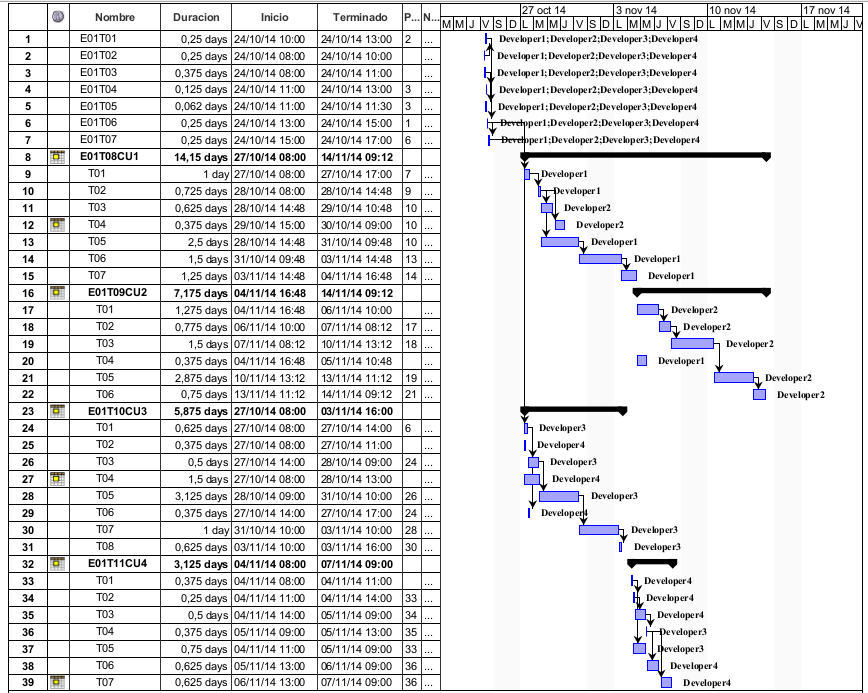
\includegraphics[width=1\textwidth]{plan.png}
  \caption{Diagrama de Gantt de la 1era iteración con la asignación de tiempo y recursos}
  \label{fig:clases4}
\end{figure}
